%versi 3 (22-07-2020)
\chapter{Landasan Teori}
\label{chap:teori}

\section{BigQuery\cite{bqa, bqIntroduction}}
Google memiliki salah satu produk yaitu BigQuery yang berbasis \textit{cloud} dan dapat digunakan untuk menganalisis data tanpa harus memikirkan database. BigQuery memaksimalkan fleksibelitas dengan memisahkan memisahkan mesin komputasi yang menganalisa data. BigQuery dapat digunakan sebagai tempat penyimpanan dan data tersebut dapat dianalisis. Data dalam BigQuery dimasukkan dalam sebuah dataset. Dataset berisikan tabel-tabel yang dapat dianalisis. Google meluncurkan BigQuery secara publik pada tahun 2012. Saat ini BigQuery sudah berkembang menjadi penyedia penyimpanan terstruktur berbasis \textit{cloud} yang dikelola dan di-\textit{hosting}. 

\subsection{\textit{Cloud Storage System}}
Selain sebagai tempat untuk menjalankan \textit{query} dari data, saat ini BigQuery juga merupakan tempat penyimpanan data terstruktur di \textit{cloud}. Data akan direplikasi ke beberapa lokasi yang berbeda secara geografis untuk meningkatkan ketersediaan dan ketahanan. Jika pusat data di Google pada suatu lokasi ditutup, data tetap dapat diakses tanpa terjadi gangguan. Data juga akan direplikasi dalam sebuah kluster agar tidak terjadi kehilangan data jika terjadi kegagalan perangkat keras. 

\subsection{\textit{SQL (Structured Query Language) \cite{book:22611}}}
SQL adalah bahasa pemograman menghasilkan, memanipulasi, dan mengambil informasi dari database relasional. BigQuery mendukung dua jenis gaya SQL yaitu \textit{Standard SQL} dan \textit{Legacy SQL} \footnote{https://cloud.google.com/bigquery/docs/reference/standard-sql/enabling-standard-sql}. Mengambil informasi dari database relasional harus menggunakan \textit{query}. \textit{Query} merupakan \textit{syntax} atau perintah yang digunakan untuk mengambil dan menghasilkan data dari database.

\subsubsection{Query Clauses}
Terdapat beberapa komponen atau klausa dari \textit{query} yang digunakan mengambil dan menghasilkan data dari database, seperti:
\begin{itemize}
    \item SELECT dan FROM\\
    Fungsi dari klausa SELECT adalah untuk menentukan kolom dari suatu tabel yang ditampilkan dalam \textit{query result}. Fungsi dari klausa FROM adalah Mengidentifikasi tabel yang ingin diambil datanya. Dalam mengambil data dari database setidaknya minimal harus menggunakan dua klausa ini. Klausa ini memiliki \textit{syntax} seperti:
    \begin{verbatim}
    SELECT coloumn1, coloumn2, ...
    FROM table_name
    \end{verbatim}
    
    \item WHERE\\
    Fungsi dari klausa WHERE adalah untuk membatasi jumlah baris dalam \textit{query result} berdasarkan kondisi tertentu. Klausa WHERE digunakan jika terdapat beberapa kondisi yang ingin dicari dari database tersebut. Klausa ini memiliki \textit{syntax} seperti:
    \begin{verbatim}
    SELECT coloumn1, coloumn2, ...
    FROM table_name
    WHERE condition
\end{verbatim}
    
    \item GROUP BY\\
    Fungsi dari klausa GROUP BY adalah untuk mengelompokkan baris berdasarkan nilai kolom yang sama. Klausa ini memiliki \textit{syntax} seperti:
    \begin{verbatim}
    SELECT coloumn1, coloumn2, ...
    FROM table_name
    WHERE condition
    GROUP BY column_name, ...
\end{verbatim}
    
    \item ORDER BY\\
    Fungsi dari klausa ORDER BY adalah untuk mengurutkan \textit{query result} berdasarkan satu atau lebih kolom. Pada saat menggunakan ORDER BY, akan ditambahkan dua fungsi yaitu ASC (\textit{Ascending}) dan DESC (\textit{Descending}). Klausa ini memiliki \textit{syntax} seperti:
    \begin{verbatim}
    SELECT coloumn1, coloumn2, ...
    FROM table_name
    WHERE condition
    GROUP BY column_name, ...
    ORDER BY column_name, ... ASC|DESC
\end{verbatim}
\end{itemize}



\subsubsection{Query Aggregation}
Didalam \textit{query} juga terdapat beberapa fungsi agregat untuk melakukan operasi tertentu yaitu:
\begin{itemize}
    \item MAX()\\
    Fungsi ini bertujuan untuk mengembalikan nilai maksimal dari atribut sebuah tabel. Fungsi MAX memiliki contoh \textit{syntax} seperti:
    \begin{verbatim}
        SELECT MAX(column_name)
        FROM table_name
        WHERE condition;
    \end{verbatim}
    
    \item MIN()\\
    Fungsi ini bertujuan untuk mengembalikan nilai minimum dari atribut sebuah tabel. Fungsi MIN memiliki contoh \textit{syntax} seperti:
    \begin{verbatim}
        SELECT MIN(column_name)
        FROM table_name
        WHERE condition;
    \end{verbatim}
    
    \item AVG()\\
    Fungsi ini bertujuan untuk mengembalikan nilai rata-rata dari atribut sebuah tabel. Fungsi AVG memiliki contoh \textit{syntax} seperti:
    \begin{verbatim}
        SELECT AVG(column_name)
        FROM table_name
        WHERE condition;
    \end{verbatim}  
    
    \item COUNT()
     Fungsi ini bertujuan untuk mengembalikan jumlah baris dari atribut sebuah tabel. Fungsi COUNT memiliki contoh \textit{syntax} seperti:
    \begin{verbatim}
        SELECT COUNT(column_name)
        FROM table_name
        WHERE condition;
    \end{verbatim} 
    
    \item SUM()
     Fungsi ini bertujuan untuk mengembalikan jumlah baris dari atribut sebuah tabel. Fungsi SUM memiliki contoh \textit{syntax} seperti:
    \begin{verbatim}
        SELECT SUM(column_name)
        FROM table_name
        WHERE condition;
    \end{verbatim} 
\end{itemize}


\subsubsection{Querying Multiple Tables}
Karena database relasional di-\textit{design} dibentuk dengan mengamanatkan bahwa setiap entitas dibuat kedalam tabel yang terpisah, sehingga dibutuhkan mekanisme untuk menghubungkan beberapa tabel dalam \textit{query} yang sama. Mekanisme ini disebut dengan JOIN. Terdapat beberapa jenis JOIN sebagai berikut:
\begin{itemize}
    \item LEFT OUTER JOIN \\
    Kata kunci kiri menunjukkan bahwa tabel di sisi kiri klausa from bertanggung jawab untuk menentukan jumlah baris dalam kumpulan hasil, sedangkan tabel di sisi kanan digunakan untuk memberikan nilai kolom setiap kali ditemukan kecocokan. LEFT OUTER JOIN memiliki \textit{syntax} seperti:
    \begin{verbatim}
        SELECT column_name(s)
        FROM table1
        LEFT (OUTER) JOIN table2
        ON table1.column_name = table2.column_name;
    \end{verbatim}
    
    \item RIGHT OUTER JOIN \\
    Kata kunci kiri menunjukkan bahwa tabel di sisi kanan klausa from bertanggung jawab untuk menentukan jumlah baris dalam kumpulan hasil, sedangkan tabel di sisi kiri digunakan untuk memberikan nilai kolom setiap kali ditemukan kecocokan. RIGHT OUTER JOIN memiliki \textit{syntax} seperti:
    \begin{verbatim}
        SELECT column_name(s)
        FROM table1
        RIGHT (OUTER) JOIN table2
        ON table1.column_name = table2.column_name;
    \end{verbatim}
    
    \item FULL OUTER JOIN \\
    Full outer join merupakan gabungan dari LEFT OUTER JOIN dan RIGHT OUTER JOIN. FULL OUTER JOIN memiliki \textit{syntax} seperti:
    \begin{verbatim}
        SELECT column_name(s)
        FROM table1
        FULL OUTER JOIN table2
        ON table1.column_name = table2.column_name
        WHERE condition;
    \end{verbatim}
    
    \item INNER JOIN \\
    Inner join menghubungkan dua atau lebih tabel dengan hubungan antara dua kolom. INNER JOIN memiliki \textit{syntax} seperti:
    \begin{verbatim}
        SELECT column_name(s)
        FROM table1
        INNER JOIN table2
        ON table1.column_name = table2.column_name;
    \end{verbatim}
\end{itemize}

\subsubsection{Subquery}
\textit{Subquery} merupakan \textit{query} yang yang terkandung dalam \textit{query} lain. Sebuah \textit{subquery} selalu diapit dalam tanda kurung, dan biasanya dieksekusi terlebih dahulu sebelum \textit{query} yang memuatnya. Tabel yang dikembalikan oleh \textit{subquery} menentukan bagaimana tabel tersebut dapat digunakan dan operator mana yang dapat digunakan oleh \textit{query} yang memuatnya untuk berinteraksi dengan tabel yang dikembalikan oleh \textit{subquery}. Ketika \textit{query} yang memuat telah selesai dieksekusi, tabel yang dikembalikan oleh \textit{subquery} akan dibuang, membuat \textit{subquery} bertindak seperti tabel sementara dengan cakupan pernyataan. Salah satu \textit{syntax} pada \textit{subquery} adalah sebagai berikut:
\begin{verbatim}
    SELECT column_name(s)
    FROM (subquery)
\end{verbatim}

\section{HTTP Archive \cite{httparchiveAbout}}
HTTP Archive adalah sebuah \textit{open-source project} yang melihat bagaimana \textit{website} dibuat. HTTP Archive menyediakan data-data historis untuk melihat bagaimana \textit{website} berkembang. HTTP Archive pertama sekali dimulai pada tahun 2010 oleh Steve Souders dan di-\textit{maintain} oleh Pat Meenan, Rick Viscomi, Paul Calvano, and Barry Pollard. Data url HTTP Archive didapatkan menggunakan CrUX kemudian url dikirimkan ke WebPageTest setiap bulannya. 
CrUX adalah sebuah dataset yang bersifat publik yang berisi data user experience dari jutaan website. Data ini berasal dari data yang dikumpulkan dari pengguna yang telah memilih untuk mengsinkronkan \textit{browsing history} mereka. Data yang dihasilkan tersedia melalui:
\begin{enumerate}
	\item PageSpeed Insights
	\item Public Google BigQuery Project
	\item CrUX Dashboard on Data Studio 
\end{enumerate} 
Orang yang menggunakan HTTP Archive adalah anggota komunitas web, para sarjana, dan pemimpin industri:
\begin{itemize}
    \item Komunitas web menggunakan data ini untuk mempelajari lebih lanjut tentang keadaan web. Biasanya dapat dilihat pada blog, presentasi, atau media sosial. 
    \item Para sarjana mengutip data ini untuk mendukung penelitian dalam publikasi besar seperti ACM dan IEEE.
    \item Para pemimpin industri menggunakan data ini untuk mengkalibrasi alat mereka untuk secara akurat mewakili bagaimana web dibuat.
\end{itemize}
Di dalam HTTP Archive terdapat dataset yang dapat diambil menggunakan teknologi BigQuery. Dataset dari HTTP Archive masih kotor sehingga terdapat beberapa data yang ganda dan terdapat versi dari aplikasi yang tidak dapat ditentukan (hanya berisi karakter atau simbol). Dataset tersebut adalah sebagai berikut:
\begin{enumerate}
	\item almanac\\
	Tabel ini tidak digunakan dalam pengerjaan skripsi ini.
	\item blink$\_$feature\\
	Tabel ini tidak digunakan dalam pengerjaan skripsi ini.
	\item core$\_$web$\_$vitals\\
	Tabel ini tidak digunakan dalam pengerjaan skripsi ini.
	\item latest\\
	Tabel ini tidak digunakan dalam pengerjaan skripsi ini.
	\item lighthouse\\
	Tabel ini tidak digunakan dalam pengerjaan skripsi ini.
	\item pages\\
	Tabel ini tidak digunakan dalam pengerjaan skripsi ini.
	\item requests\\
	Tabel ini tidak digunakan dalam pengerjaan skripsi ini.
	\item response$\_$bodies\\
	Tabel ini tidak digunakan dalam pengerjaan skripsi ini.
	\item sample$\_$data\\
	Tabel ini tidak digunakan dalam pengerjaan skripsi ini.
	\item sample$\_$data$\_$2020\\
	Tabel ini tidak digunakan dalam pengerjaan skripsi ini.
	\item scratchspace\\
	Tabel ini tidak digunakan dalam pengerjaan skripsi ini.
	\item summary$\_$pages\\
	Tabel ini tidak digunakan dalam pengerjaan skripsi ini.
	\item summary$\_$requests\\
	Tabel ini tidak digunakan dalam pengerjaan skripsi ini.
	\item technologies\\
	Dataset pada technologies berisi tabel-tabel dari bulan Januari tahun 2016 sampai dengan sekarang yang terdiri dari website pada desktop dan mobile. Dataset bulan Agustus tahun 2020 baris pada desktop memiliki 61.203.638 baris 
	 %Contoh data dapat dilihat pada tabel \ref{table:ct_tech_desktop} 
	 dan pada mobile memiliki 67.452.994 baris. 
	 %Contoh data dapat dilihat pada tabel \ref{table:ct_tech_mobile}. Masing-masing terdiri dari 4 kolom yaitu \textit{url}, \textit{category}, \textit{app}, \textit{info}. Pada kolom \textit{URL (Uniform Resource Locator)} merupakan nama-nama domain, \textit{category} merupakan jenis aplikasi yang digunakan pada website tersebut, \textit{app} merupakan aplikasi yang digunakan website tersebut, \textit{info} merupakan informasi tambahan dari aplikasi. 
	\item urls\\
	Tabel ini tidak digunakan dalam pengerjaan skripsi ini.
	\item wappalyzer\\
	Tabel ini tidak digunakan dalam pengerjaan skripsi ini.
\end{enumerate}



% \section{Web Almanac \cite{webalmanacMetho}}
% Web Almanac adalah sebuah project yang dikelola oleh HTTP Archive. Misi web almanac adalah membuat gudang data untuk HTTP ARchive agar dapat diakses dengan mudah oleh komunitas web. Semua metrik yang disediakan oleh web almanac dapat direproduksi secara publik menggunakan dataset di BigQuery. Kueri dapat ditelusuri dengan menggunakan semua bab di repositori GitHub web almanac yang dapat dilihat pada \footnote{https://github.com/HTTPArchive/almanac.httparchive.org/tree/main/sql/2020}: 
% \begin{enumerate}
%     \item Accessibility\\
%     Aksesibilitas web adalah tentang pencapaian fitur dan informasi serta memberikan akses lengkap ke semua aspek antarmuka bagi orang yang tidak memiliki akses. Sebuah produk digital atau situs web tidak lengkap jika tidak dapat digunakan oleh semua orang. 
%     \item Caching\\
%     Caching adalah teknik yang memungkinkan penggunaan kembali konten yang diunduh sebelumnya. Caching melibatkan sesuatu seperti server atau web browser untuk menyimpan konton dan menandainya agar dapat digunakan kembali.
%     \item Capabilities\\
%     Capabilties memberikan \textit{overview} tentang berbagai API web modern. Hal ini penting untuk menjaga web tetap relevan sebagai platform. 
%     \item CMS\\
%     Istilah CMS mengacu pada sistem yang memungkinkan individu dan organisasi untuk membuat, mengelola, dan mempublikasikan konten. CMS pada konton web adalah sistem yang bertujuan untuk membuat, mengelola, dan menerbitkan konten untuk dikonsumsi dan dialami melalui internet.
%     \item Compression\\
%     Menggunakan HTTP Compression membuat pemuatan situs lebih cepat dan menjamin pengalaman penggunaan yang lebih baik. Penggunaan compression yang efektif dapat mengurangi berat halaman dan meningkatkan kinerja web.
%     \item CSS\\
%     CSS adalah bahasa yang digunakan untuk membuat tampilan dan format pada web dan media lainnya.
%     \item Ecommerce\\
%     Ecommerce platform adalah perangkat lunak atau layanan yang memungkinkan untuk membuat dan mengoperasikan sebuah toko online.
%     \item Fonts\\
%     Fonts adalah bagian penting dalam sebuah situs web dan tipografi adalah seni menyajikan teks tersebut dengan cara yang menarik dan efektif secara visual. Dalam pembuatan tipografi yang baik dibutuhkan pemilihan font yang sesuai. Dalam hal ini akan ditunjukkan bagaimana font web digunakan dan bagaimanafont tersebut dioptimalkan. 
%     \item HTTP\\
%     HTTP adalah protokol lapisan aplikasi yang dirancang untuk mentransfer informasi antara perangkat jaringan dan berjalan di atas lapisan lain dari tumpukan protokol jaringan. Dalam web almanac akan mengulas bagaimana status penerapan HTTP/2 atau HTTP versi dua pada saat ini.
%     \item Jamstack\\
%     Jamstack adalah konsep arsitektur yang relatif baru yang dirancang untuk membuat web lebih cepat, lebih aman, dan lebih mudah untuk diskalakan. Dalam web almanac akan memperkirakan dan menganalisis pertumbuhan situs Jamstack, kinerja kerangka kerja Jamstack populer, serta analisis pengalaman pengguna nyata menggunakan metrik Core Web Vitals.
%     \item Javascript\\
%     JavaScript adalah bahasa pemograman yang digunakan untuk menentukan perilaku. 
%     \item Markup\\
%     HTML adalah dasar dari sebuah \textit{website} yang akan ditampilkan ke-\textit{user}. Dalam web almanac mengacu pada kumpulan halaman \textit{mobile}.
%     \item Media\\
%     Pada web alamanac, media digunakan untuk menganalisa bagaimana menggunakan gambar dan video di web.
%     \item Mobile-web\\
%     Saat ini, mobile-web sudah menjadi cara utama banyak orang untuk mengakses \textit{website}. Dalam mobile-web akan terlihat tren saat ini pada mobile-web.
%     \item Page-weight\\
%     Page-weight adalah salah satu metrik sederhana yang tersedia. Memuat sebuah halaman akan memberikan gambaran tentang ukuran dari \textit{resource} yang diambil atau di-\textit{request}.    \item Performance\\
%     Dalam web almanac, akan melihat data kinerja di dunia nyata yang disediakan oleh Laporan Pengalaman Pengguna Chrome (CrUX) melalui lensa perkembangan baru tersebut serta menganalisis beberapa metrik relevan lainnya.
%     \item Privacy\\
%     Web almanac memberikan gambaran umum tentang keadaan privasi saat ini di web. Hal ini bertujuan untuk meningkatkan akuntabilitas pemroses data dan transparansi mereka terhadap pengguna. Dalam hal ini, kami membahas prevalensi pelacakan online dengan berbagai teknik dan tingkat adopsi spanduk persetujuan cookie dan kebijakan privasi oleh situs web.
%     \item PWA\\
%     Dalam web almanac, kita akan melihat setiap komponen yang membuat PWA seperti apa adanya, dari perspektif berbasis data.
%     \item Resource-hints\\
%     % Dalam web almanac, \textit{resource hints} berguna untuk mendefinisikan hubungan dns-prefetch, preconnect, prefetch, dan prerender dari \textit{HTML Link Element}. 
%     \item Security\\
%     Dalam web almanac, akan dilakukan menganalisis penerapan berbagai fitur keamanan secara mendalam dan dalam skala besar, kami mengumpulkan wawasan tentang berbagai cara pemilik situs web menerapkan mekanisme keamanan ini, didorong oleh insentif untuk melindungi penggunanya.
%     \item SEO\\
%     Dalam web almanac, untuk mengidentifikasi dan menilai elemen dan konfigurasi utama yang berperan dalam pengoptimalan pencarian organik situs web.
%     \item Third-parties\\
%     Web almanac meninjau prevalensi konten pihak ketiga dan bagaimana hal ini telah berubah sejak 2019.
% \end{enumerate}



\section{Pengukuran Aplikasi Usang Pada Beberapa \textit{Website} Populer Di Indonesia\cite{pascal}}

Pada jurnal ini menjelaskan bahwa dalam bidang keamanan komputer, terdapat berbagai jenis metode dalam menyerang kerentanan pada sebuah sistem. Pengelola sistem yang sudah terkena dampak harus memperbarui sistemnya. Penelitian ini mengusulkan metode untuk melakukan pengukuran website tentang seberapa banyak penggunaan aplikasi yang tidak didukung. Pada penelitian ini dibataskan pada mendeteksi versi aplikasi yang digunakan.

\subsection{\textit{Research Method}}
Terdapat empat langkah dalam meelakukan penelitian ini, yaitu:
\begin{enumerate}
    \item Memilih list \textit{website} yang populer\\
    Memilih \textit{website} paling populer dilakukan dengan mengambil daftar dari \textit{website} teratas dari Alexa dengan negara tertentu.
    \item Mengidentifikasi aplikasi yang dipakai \textit{website}\\
    Untuk setiap \textit{website} akan dilakukan pengidentifikasian nomor versi yang dipakai. Hal ini dibantu dengan menggunakan \textit{third party} yaitu Wappalyzer. 
    \item Mengelompokkan berdasarkan nama aplikasi dan ambil versi yang didukung\\
    Untuk melihat nomor versi yang masih didukung akan dilakukan pencarian di \textit{website} resmi dari setiap aplikasi. Terdapat beberapa \textit{website} yang tidak dapat ditampilkan versinya, sehingga suatu \textit{website} dapat didefinisikan didukung jika memenuhi kondisi sebagai beikut:
    \begin{itemize}
        \item Versi aplikasi yang didukung dapat dilihat secara eksplisit di dalam \textit{website}.
        \item Dokumen untuk versi aplikasi tersebut masih tersedia.
        \item Aplikasi secara langsung memberikan pernyataan untuk versi yang masih didukung.
    \end{itemize}
    
    \item Membandingkan versi yang dipakai aplikasi saat ini dengan versi aplikasi yang didukung dapat dilihat pada gambar \ref{fig:apr}\\
    Buka kembali setiap aplikasi kemudian menggunakan Wappalyzer untuk membandingkan versi aplikasi yang dipakai dengan versi aplikasi yang masih didukung. Klasifikasikan setiap aplikasi di setiap situs web menjadi salah satu dari berikut ini:
    \begin{itemize}
        \item \textit{Not-versioned} berarti aplikasi yang terdeteksi oleh Wappalyzer tidak memiliki informasi versi sehingga tidak dapat dibandingkan.
        \item Non-konklusif dapat berarti salah satu dari dua:
        \begin{itemize}
            \item Dapat mengambil nomor versi yang digunakan dalam aplikasi, tetapi kami tidak dapat menentukan apakah versi tersebut masih didukung atau tidak oleh pengelola.
            \item Versi yang didukung untuk aplikasi tertentu tidak diketahui.
        \end{itemize}
        \item Tidak didukung berarti dapat disimpulkan bahwa aplikasi yang digunakan menggunakan nomor versi yang tidak didukung oleh pengelola.
        \item Didukung berarti dapat disimpulkan bahwa aplikasi yang digunakan menggunakan nomor versi masih didukung oleh pengelola.
    \end{itemize}
    \begin{figure}[H]
	\centering  
	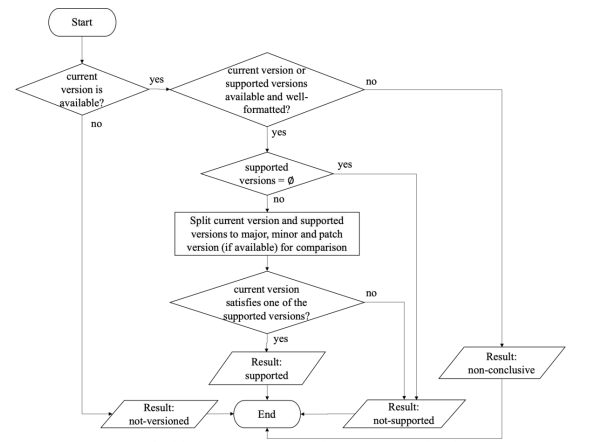
\includegraphics[scale=0.9]{Gambar/compare_version.PNG}  
	\caption{\textit{Algoritma untuk membandingkan versi yang dipakai dengan versi yang masih didukung}} 
	\label{fig:apr} 
\end{figure}
\end{enumerate}


\subsection{Hasil Keseluruhan}
Pada jurnal\cite{pascal}, dari 1.500 URL yang dideteksi oleh Wappalyzer, hanya 1.439 URL yang berhasil diidentifikasi. Dari 1.500 URL terebut ditemukan total 12.762 aplikasi yang dapat dilihat pada tabel \ref{table:apr}
\begin{table}[h!]
\centering
\begin{tabular}{lrr} 
 \hline
 \textbf{Result} & \textbf{Application count} & \textbf{Percentage}\\
 \hline
 Not-versioned & 8,980 & 70.37\\
 Non-conclusive & 1,409 & 11.04\\
 Unsupported & 1,508 & 11.82\\
 Supported & 865 & 6.78\\
 \hline
 Total & 12,762 & 100.00\\
 \hline

\end{tabular}
\caption{Jumlah keseluruhan aplikasi berdasarkan hasil pengukuran}
\label{table:apr}
\end{table}

Tabel \ref{table:first-ten} adalah daftar sepuluh website yang paling popular. Dari daftar tersebut terlihat banyak sekali website yang menggunakan aplikasi yang tidak ada informasi versinya. Tetapi untuk yang ada informasi versinya, terdapat beberapa aplikasi yang sudah tidak didukung. Beberapa aplikasi yang sudah tidak didukung dari sepuluh website tersebut adalah Bootstrap, Font Awesome, jQuery, dan PHP. Pada tabel \ref{table:n-result} terdapat 1,500 website yang dipisahkan setiap 150 website yang diurutkan berdasarkan rank website tersebut. Untuk setiap baris pada tabel tersebut akan dihitung website yang menggunakan n aplikasi yang sudah tidak didukung. 
\begin{table}[H]
	\centering
	\begin{tabular}{rlcccc} 
		\hline
		\textbf{rank} & \textbf{domain name} & \textbf{not-versioned} & \textbf{non-conclusive} & \textbf{unsupported} & \textbf{supported}\\
		\hline
		1 & okezone.com & 7&0&1&1\\
		\hline
		2 & google.com & 1&0&0&0\\
		\hline
		3 & tribunnews.com & 11&2&2&0\\
		\hline
		4 & youtube.com & 1&1&0&0\\
		\hline
		5 & grid.id & 11&1&2&1\\
		\hline
		6 & detik.com & 8&3&0&0\\
		\hline
		7 & kompas.com & 10&2&1&0\\
		\hline
		8 & sindonews.com & 4&1&1&0\\
		\hline
		9 & tokopedia.com & 5&0&0&0\\
		\hline
		10 & liputan6.com & 11&1&1&0\\
		\hline
\end{tabular}
\caption{Sepuluh Hasil Pengukuran}
\label{table:first-ten}
\end{table}

\begin{table}[H]
	\centering
	\begin{tabular}{rccccc} 
		\hline
		\textbf{rank} & \textbf{r=0} & \textbf{r=1} & \textbf{r=2} & \textbf{r=3} & \textbf{r=4}\\
			\hline
			1-150 & 56 & 58&26&9&1\\
			\hline
			151-300 & 52 & 55&29&12&2\\
			\hline
			301-450 & 59 & 43&32&10&6\\
			\hline
			451-600 & 56 & 48&22&21&3\\
			\hline
			601-750 & 59 & 58&22&10&1\\
			\hline
			751-900 & 68 & 44&25&8&5\\
			\hline
			901-1,050 & 65 & 42&30&10&3\\
			\hline
			1,051-1200 & 56 & 46&34&10&4\\
			\hline
			1201-1,350 & 50 & 57&31&11&1\\
			\hline
			1,350-1,500 & 62 & 46&29&11	&2\\
			\hline
		\end{tabular}
		\caption{Jumlah aplikasi yang tidak didukung berdasarkan rank website}
		\label{table:n-result}
	\end{table}

Pada tabel \ref{table:most-used}, terdapat beberapa aplikasi yang banyak digunakan. Beberapa aplikasi tersebut diambil dari 1.500 \textit{website} teratas dan memfilter aplikasi yang versinya tidak dapat diidentifikasi di salah satu dari 1.500 \textit{website} teratas.
\begin{table}[H]
	\centering
	\begin{tabular}{rlcccc} 
		\hline
		\textbf{numsites} & \textbf{name} & \textbf{supported} & \textbf{unsupported} & \textbf{non-conclusive} & \textbf{not-versioned}\\
		\hline
		1,011 & jQuery & 260&737&0&14\\
		\hline
		591 & PHP & 118&127&0&346\\
		\hline
		478 & Nginx & 5&116&0&357\\
		\hline
		430 & Bootstrap & 114&228&0&88\\
		\hline
		400 & Font Awesome & 70&157&13&160\\
		\hline
		346 & WordPress & 118&41&6&181\\
		\hline
		298 & jQuery Migrate & 0&0&267&31\\
		\hline
		237 & Apache & 79&10&2&146	\\
		\hline
	\end{tabular}
	\caption{Aplikasi yang Banyak Digunakan}
	\label{table:most-used}
\end{table}

\section{ReactJS}
ReactJS merupakan \textit{library} yang disediakan JavaScript untuk membuat \textit{interface}. ReactJS dibuat oleh Facebook. 
%Berikut ini contoh sintaks pada ReactJS:
%\begin{lstlisting}
%    class HelloMessage extends React.Component {
%  render() {
%    return (
%      <div>
%        Hello {this.props.name}
%      </div>
%    );
%  }
%}
%
%ReactDOM.render(
%  <HelloMessage name="World" />,
%  document.getElementById('hello-example')
%);
%\end{lstlisting}

\subsection{JSX}
JSX adalah sebuah ekstensi Javascript yang dapat mengikutsertakan HTML dalam Javascript. JSX akan menghasilkan "elemen" React. 
\subsubsection{Menyatukan Ekspresi dalam JSX}
Berikut ini adalah contoh penggunaan JSX:
\begin{lstlisting}
	const name = 'Budi';
	const element = <h1>Halo, {name}</h1>;
	
	ReactDOM.render(
	element,
	document.getElementById('root')
	);
\end{lstlisting}
Pada contoh diatas, variabel name akan dibungkus dengan menggunakan tanda kurung kurawal. Semua ekspresi Javascript valid dalam tanda kurung kurawal di JSX. 
\subsubsection{Mengspesifikasikan Atribut Dengan JSX}
Penulis dapat menggunakan tanda petik untuk mengspesifikasikan string literal sebagai atribut:
\begin{lstlisting}
	const element = <a href="https://www.reactjs.org"> link </a>;
\end{lstlisting}
 Penulis juga dapat menggunakan kurung kurawal untuk mengspesifikasikan ekspresi Javascript di dalam atribut:
 \begin{lstlisting}
 	const element = <img src={user.avatarUrl}></img>;
 \end{lstlisting}

\subsubsection{Mengspesifikasikan Elemen Anak dengan JSX}
Jika tag bersifat kosong atau tidak memiliki elemen anak, penulis dapat menutup tag-nya secara langsung dengan />, seperti pada potongan kode dibawah ini.
\begin{lstlisting}
	const element = <img src={user.avatarUrl} />;
\end{lstlisting}
Didalam tag JSX memungkinkan untuk memiliki elemen anak, yang dapat dilihat pada potongan kode dibawah ini.
\begin{lstlisting}
	const element = (
	<div>
	<h1>Halo!</h1>
	<h2>Senang melihatmu di sini.</h2>
	</div>
	);
\end{lstlisting}

\subsection{Merender Elemen}
Sebuah elemen menggambarkan hal yang ingin ditampilkan pada layar. Tidak seperti elemen DOM, elemen React merupakan objek biasa dan mudah dibuat. React DOM mangatur pembaruan DOM agar sesuai dengan elemen React.
\subsubsection{Me-render Elemen Kedalam DOM}
Aplikasi yang dibuat dengan React biasanya memiliki satu node DOM akar. Jika mengintegrasikan React ke dalam aplikasi yang sudah ada, penulis dapat memiliki node DOM akar yang terisolasi sebanyak yang Anda inginkan.
\begin{lstlisting}
	<div id="root"></div>
\end{lstlisting}
Potongan kode diatas disebut sebagai node DOM akar karena semua yang berada didalamnya akan diatur oleh React DOM.
\begin{lstlisting}
	const element = <h1>Hello, world</h1>;
	ReactDOM.render(element, document.getElementById('root'));
\end{lstlisting}
Pada kode diatas, elemen dan root dimasukkan kedalam ReactDOM.render() agar elemen tersebut dapat dirender.
\subsubsection{Memperbarui Elemen yang Di-render}
Elemen React bersifat \textit{immutable} sehingga setelah elemen dibuat, penulis tidak dapat mengubah nilai dari elemen atau attributnya. Satu-satunya cara untuk memperbarui antarmukanya adalah dengan membuat elemen baru atau menggunakan ReactDOM.render()
\begin{lstlisting}
	function tick() {
		const element = (
		<div>
		<h1>Hello, world!</h1>
		<h2>It is {new Date().toLocaleTimeString()}.</h2>
		</div>
		);
		ReactDOM.render(element, document.getElementById('root'));
	}
	
	setInterval(tick, 1000);
\end{lstlisting}
Pada kode diatas ReactDOM.render() membuat \textit{callback} setiap detik.

\subsection{Components and Props}
Komponen mempermudah untuk memisahkan antarmuka menjadi bagian tersendiri dan dapat digunakan kembali. Secara konsep, komponen menyerupai fungsi Javascript. Komponen dapat menerima beberapa props (masukan) dan mengembalikan elemen React yang mendeskripsikan apa yang seharusnya tampil dilayar. 
\subsubsection{Fungsi dan Komponen Kelas}
Cara yang paling sederhana untuk mendefinisikan sebuah komponen adalah dengan menuliskan sebuah fungsi Javascript
\begin{lstlisting}
	function Welcome(props) {
		return <h1>Halo, {props.name}</h1>;
	}
\end{lstlisting}
Fungsi diatas adalah contoh komponen React yang sah karena menerima sebuah props tunggal atau argumen objek dengan data dan kembalian sebuah elemen React. 

\subsubsection{Merender Sebuah Komponen}
Didalam React Elemen dapat mewakili komponen yang didefinisikan oleh penulis. Seperti pada kode dibawah.
\begin{lstlisting}
	const element = <Welcome name="Sara" />;
\end{lstlisting}
Ketika React melihat sebuah elemen mewakili sebuah komponen yang dibuat oleh penulis, komponen akan mengoper atribut JSX ke dalam komponen ini sebagai objek tunggal. Objek ini disebut sebagai props. Kode dibawah ini akan menghasilkan "Halo Sara" pada halaman.
\begin{lstlisting}
	function Welcome(props) {
		return <h1>Halo, {props.name}</h1>;
	}
	
	const element = <Welcome name="Sara" />;
	ReactDOM.render(
	element,
	document.getElementById('root')
	);
\end{lstlisting} 

\subsubsection{Menyusun Komponen}
Komponen dapat merujuk ke komponen lain pada keluarannya. Hal ini memungkinkan kita untuk membuat abstraksi dari komponen yang sama untuk tingkat detail. Seperti membuat sebuah tombol, sebuah form, sebuah tampilan, sebuah dialog. Dalam aplikasi React, semua itu dinyatakan dalam bentuk komponen. Sebagai contoh penulis dapat membuat sebuah komponen App yang mencetak Welcome berkali-kali.
\begin{lstlisting}
	function Welcome(props) {
		return <h1>Halo, {props.name}</h1>;
	}
	
	function App() {
		return (
		<div>
		<Welcome name="Sara" />
		<Welcome name="Cahal" />
		<Welcome name="Edite" />
		</div>
		);
	}
\end{lstlisting}

%\subsection{State dan Lifecycle}


\subsection{Penanganan Event}
Menangani events dengan elemen React sangat mirip seperti menangani sebuah events pada elemen DOM. Ada beberapa perbedaan sintaks:
\begin{itemize}
	\item Events pada React biasanya ditulis dalam bentuk camelCase, bukan lowercase.
	\item Dengan JSX Anda dapat mengoper function sebagai event handler, bukan sebagai string.
\end{itemize}
Berikut ini adalah contoh sintaks pada HTML:
\begin{lstlisting}
	<button onclick="activateLasers()">
	Aktivasi Laser
	</button>
\end{lstlisting}
Sintaks HTML memiliki sedikit perbedaan dengan sintaks pada React. Berikut ini adalah contoh sintaks pada React:
\begin{lstlisting}
	<button onClick={activateLasers}>
	Aktivasi Laser
	</button>
\end{lstlisting} 
Perbedaan lainnya adalah penulis tidak dapat mengembalikan nilai false untuk mencegah behaviorbawaan React. Penulis harus menggunakan preventDefault. Sebagai contoh, pada HTML untuk mencegah agar link bawaan membuka halaman baru, penulis dapat menulis seperti ini:  
\begin{lstlisting}
	<a href="#" onclick="console.log('The link was clicked.'); return false">
	Click me
	</a>
\end{lstlisting}
Sedangkan pada React, contoh tersebut dapat ditulis sebagai berikut:
\begin{lstlisting}
	function ActionLink() {
		function handleClick(e) {
			e.preventDefault();
			console.log('Tautan diklik.');
		}
		
		return (
		<a href="#" onClick={handleClick}>
		Klik Saya
		</a>
		);
	}
\end{lstlisting}
Pada kode diatas e merupakan event tiruan. React mendefinisikan event tiruan ini berdasarkan W3C spec\footnote{https://www.w3.org/TR/DOM-Level-3-Events/}, jadi Anda tidak perlu khawatir akan kesesuaian antar lintas browser. Event dalam React tidak bekerja secara sama dengan event native dari $\_$browser.
\subsubsection{Mengoper Argumen Kedalam Penanganan Event}
Di dalam perulangan, umumnya Anda ingin mengoper sebuah parameter ekstra kedalam penanganan event. Sebagai contoh, jika id sama dengan ID baris, maka salah satu dari kedua contoh berikut dapat dijalankan:
\begin{lstlisting}
	<button onClick={(e) => this.deleteRow(id, e)}>Delete Row</button>
	<button onClick={this.deleteRow.bind(this, id)}>Delete Row</button>
\end{lstlisting}
Dua baris di atas memiliki arti yang sama, masing-masing menggunakan arrow functions dan Function.prototype.bind.
Arrow function adalah sebuah cara alternatif untuk mendefinisikan fungsi dari fungsi tradisional. Cara ini bersifat terbatas dan tidak dapat digunakan dalam setiap kondisi. Sedangkan metode bind() adalah sebuah metode yang membuat sebuah fungsi yang ketika dipanggil, kata kunci this akan berubah menjadi nilai yang diberikan.

\subsection{Render Bersyarat}
Render bersyarat pada React memiliki fungsi yang sama dengan operator bersyarat pada Javascript. Pada Javascript operator if atau operator bersyarat digunakan untuk merepresentasikan elemen pada state tertentu, kemudian React akan memperbarui UI pada state tersebut.

Contoh nya seperti dua komponen berikut ini:
\begin{lstlisting}
	function UserGreeting(props) {
		return <h1>Welcome back!</h1>;
	}
	
	function GuestGreeting(props) {
		return <h1>Please sign up.</h1>;
	}
\end{lstlisting}
Komponen diatas akan digunakan untuk melakukan Greetings berdasarkan pada apakah user sudah melakukan login:
\begin{lstlisting}
	function Greeting(props) {
		const isLoggedIn = props.isLoggedIn;
		if (isLoggedIn) {
			return <UserGreeting />;
		}
		return <GuestGreeting />;
	}
	
	ReactDOM.render(
	// Try changing to isLoggedIn={true}:
	<Greeting isLoggedIn={false} />,
	document.getElementById('root')
	);
\end{lstlisting} 

\subsection{List dan Keys}
Javascript dapat menggunakan fungsi map() untuk mengambil array numbers dan menggandakan angkanya. Map() akan mengembalikan nilai dalam bentuk array yang baru kemudian akan disimpan dalam sebuah variabel doubled.
Berikut ini adalah contoh kodenya:
\begin{lstlisting}
	const numbers = [1, 2, 3, 4, 5];
	const doubled = numbers.map((number) => number * 2);
	console.log(doubled);
\end{lstlisting}
Kode diatas akan mengembalikan nilai [2, 4, 6, 8, 10] ke dalam konsol. Pada React, mengubah array ke dalam list elemen kurang lebih sama.
\subsubsection{Me-render Banyak Komponen}
Penulis dapat membangun koleksi dari beberapa elemen dan menyertakannya dalam JSX  menggunakan tanda kurung kurawal. 
\begin{lstlisting}
	const numbers = [1, 2, 3, 4, 5];
	const listItems = numbers.map((number) =>
	<li>{number}</li>
	);
\end{lstlisting}
Pada kode diatas, akan dilakukan perulangan pada numbers yang berisi array dengan mengunakan fungsi map(). Hasil yang akan dikeluarkan adalah sebuah elemen <li> untuk setiap item yang kemudian akan dimasukkan kedalam variabel listItem. 
\begin{lstlisting}
	ReactDOM.render(
	<ul>{listItems}</ul>,
	document.getElementById('root')
	);
\end{lstlisting}
Kemudian dengan menggunakan kode diatas, array listItem tersebut dapat dimasukkan kedalam elemen <ul> dan akan me-render-nya kedalam DOM.

\subsubsection{Daftar Komponen Dasar}
Penulis dapat me-refaktor contoh sebelumnya ke dalam sebuah komponen yang menerima array numbers dan mengeluarkan sebuah list elemen yang tidak berurutan.
\begin{lstlisting}
	function NumberList(props) {
		const numbers = props.numbers;
		const listItems = numbers.map((number) =>
		<li>{number}</li>
		);
		return (
		<ul>{listItems}</ul>
		);
	}
	
	const numbers = [1, 2, 3, 4, 5];
	ReactDOM.render(
	<NumberList numbers={numbers} />,
	document.getElementById('root')
	);
\end{lstlisting}
Ketika penulis menjalankan kode ini, penulis akan mendapatkan peringatan bahwa key harus disediakan untuk item di dalam list. Sebuah ”key” adalah atribut string spesial yang perlu disertakan dalam pembuatan list elemen. Penulis harus sertakan key ke dalam list item pada numbers.map() dan memperbaiki masalah key yang hilang.
\begin{lstlisting}
	function NumberList(props) {
		const numbers = props.numbers;
		const listItems = numbers.map((number) =>
		<li key={number.toString()}>
		{number}
		</li>
		);
		return (
		<ul>{listItems}</ul>
		);
	}
	
	const numbers = [1, 2, 3, 4, 5];
	ReactDOM.render(
	<NumberList numbers={numbers} />,
	document.getElementById('root')
	);
\end{lstlisting}
\subsubsection{Key}
Key membantu React untuk mengidentifikasi item mana yang telah diubah, ditambahkan, atau dihilangkan. Key harus diberikan di dalam elemen yang terdapat di dalam sebuah array untuk memberikan elemen tersebut identitas yang stabil:
\begin{lstlisting}
	const numbers = [1, 2, 3, 4, 5];
	const listItems = numbers.map((number) =>
	<li key={number.toString()}>
	{number}
	</li>
	);
\end{lstlisting}
Cara terbaik untuk menentukan key yang akan digunakan adalah menggunakan string unik untuk mengidentifikasikan item. Biasanya menggunakan ID dari data sebagai key:
\begin{lstlisting}
	const todoItems = todos.map((todo) =>
	<li key={todo.id}>
	{todo.text}
	</li>
	);
\end{lstlisting}
Ketika tidak memiliki ID yang stabil untuk me-render item, penulis dapat menggunakan indeks dari item sebagai key untuk pilihan terakhir:
\begin{lstlisting}
	const todoItems = todos.map((todo, index) =>
	<li key={index}>
	{todo.text}
	</li>
	);
\end{lstlisting}

\subsection{Form}
Elemen form HTML bekerja sedikit berbeda dari elemen DOM lainnya di React, karena elemen form secara natural menyimpan beberapa state internal. Sebagai contoh, form ini pada HTML biasa menerima nama tunggal:
\begin{lstlisting}
	<form>
	<label>
	Name:
	<input type="text" name="name" />
	</label>
	<input type="submit" value="Submit" />
	</form>
\end{lstlisting}
Form ini memiliki perilaku dasar dari form HTML biasa yakni menuju ke laman baru ketika user mengirim form tersebut. Jika Anda menginginkan perilaku seperti ini di React, ini sebenarnya dapat bekerja. Namun di banyak kasus, akan lebih mudah untuk memiliki sebuah fungsi JavaScript yang menangani sebuah submisi dari sebuah form dan memiliki akses terhadap data yang dimasukkan pengguna ke dalam form. Cara standar untuk mencapai hal ini adalah dengan teknik yang disebut ”controlled component“.
\subsubsection{Controlled Component}
Elemen form pada HTML seperti <input>, <select>, dan <textarea> biasanya menyimpan state mereka sendiri dan memperbaruinya berdasarkan masukkan dari pengguna. Pada React, state yang dapat berubah akan disimpan dalam sebuah prop atau komponen dan hanya dapat diubah dengan menggunakan setState(). 
komponen React yang me-render sebuah form juga mengontrol hal yang terjadi dalam form tersebut pada masukan pengguna selanjutnya. Sebuah elemen masukan form yang nilainya dikontrol oleh React melalui cara seperti ini disebut sebagai ”controlled component“.
\begin{lstlisting}
	class NameForm extends React.Component {
		constructor(props) {
			super(props);
			this.state = {value: ''};
			
			this.handleChange = this.handleChange.bind(this);
			this.handleSubmit = this.handleSubmit.bind(this);
		}
		
		handleChange(event) {
			this.setState({value: event.target.value});
		}
		
		handleSubmit(event) {
			alert('A name was submitted: ' + this.state.value);
			event.preventDefault();
		}
		
		render() {
			return (
			<form onSubmit={this.handleSubmit}>
			<label>
			Name:
			<input type="text" value={this.state.value} onChange={this.handleChange} />
			</label>
			<input type="submit" value="Submit" />
			</form>
			);
		}
	}
\end{lstlisting}
Dengan sebuah controlled component, nilai input akan selalu didorong oleh state di React. Meskipun menulis kode yang lebih banyak, tetapi juga bisa mengoper nilai ini ke elemen antarmuka lain, atau me-reset nilai tersebut dari event handler lain.
\subsubsection{Mengendalikan Nilai Kosong}
Menentukan nilai prop pada controlled component mencegah pengguna mengubah masukan. Jika sudah menetepkan nilai value tetapi masukan masih dapat diubah, mungkin nilai value yang ditetapkan bersifat undefined atau null.


%\subsection{Memindahkan State Ke Atas}


%\subsection{Komposisi Dan Perwarisan}


\subsection{\textit{Node Package Manager}}
Node \textit{Package} Manager (NPM) adalah \textit{software registry} yang digunakan untuk meminjam atau membagikan \textit{software library} \cite{npmAbout}. NPM terdiri dari tiga komponen penting, yaitu:
\begin{itemize}
    \item NPM \textit{website}.
    \item NPM CLI ( \textit{Command Line Interface}). 
    \item NPM \textit{Registry}.
\end{itemize}

Beberapa kegunaan dari menggunakan NPM adalah:
\begin{itemize}
    \item Membagikan kode kepada pengguna NPM lainnya dimanapun.
    \item Men\textit{-download software library}
    \item Menjalankan pack\textit{}age tanpa harus meng-\textit{install} npx
\end{itemize}

\subsection{NPM CLI}
NPM merupakan \textit{package manager} untuk \textit{Node JavaScript}. NPM menempatkan modul sehingga dapat ditemukan oleh \textit{node}. Selain itu NPM juga dapat mengelola \textit{dependency conflicts.} NPM digunakan untuk menginstall dan mengembangkan \textit{node program.}. Dalam penulisan NPM dapat dilakukan didalam CLI \textit{(Command Line Interface)}. NPM memiliki tiga komponen penting dalam penulisan perintah CLI, komponen tersebut seperti:
\begin{verbatim}
    npm <command> [args]
\end{verbatim}

\subsection{NPX}
NPX merupakan \textit{execute NPM package binaries}. NPX digunakan untuk menjalan \textit{command} yang dimiliki NPM. NPX mengeksekusi file \textit{binary} dari \textit{package} \textit{Node.js}, baik yang sudah terinstal maupun yang belum. Pembuatan \textit{project} react dapat dilakukan dengan menggunakan sintaks:
    \begin{verbatim}
        npx create-react-app my-app
        cd my-app
        npm start
    \end{verbatim}

\section{ChartJS}
ChartJS adalah sebuah open-source library JavaScript yang digunakan untuk visualisasi data. Tipe-tipe chart yang didukung oleh ChartJS adalah bar, line, area, pie, bubble, radar, polar, mix, dan scatter. Pada skripsi ini tipe chart yang digunakan adalah bar chart. Untuk menginstall library ChartJS dapat dilakukan dengan menggunakan sintaks:
\begin{verbatim}
	npm i react-chartjs-2 chart.js
\end{verbatim}

\section{JSON}
JSON (JavaScript Object Notation) merupakan format penulisan data yang mudah untuk dibaca manusia maupun mesin. JSON adalah format teks yang bersifat \textit{language independent} tetapi menggunakan konvensi yang akrab bagi programmer C, Java, JavaScript, Perl, Python, dan banyak lainnya. Properti ini menjadikan JSON sebagai bahasa pertukaran data yang ideal. Terdapat dua struktur dalam JSON:
\begin{itemize}
    \item Kumpulan pasangan nilai yang akan dibuat menjadi sebuah objek, \textit{hash table}, dan lainnya.
    \item Daftar nilai yang diurutkan, seperti array, vektor, dan lainnya.
\end{itemize}
